% Netzwerkanltung für die Studentenstadt Freimann
% Tex initially created by Maximilian Engelhardt <maximilian.engelhardt@stusta.mhn.de>

%\documentclass[a4paper,12pt,draft]{scrartcl}
\documentclass[a4paper,12pt]{scrartcl}

\usepackage[utf8]{inputenc}
\usepackage{ngerman}
\usepackage{eurosym}
\usepackage{tabularx}
%\usepackage[T1]{fontspec}
%\usepackage{newcomputermodern}
\renewcommand*{\familydefault}{\sfdefault}
\usepackage[pdftex,final]{graphicx}
\usepackage[top=1.5cm,bottom=2.5cm,left=1.5cm,right=1.5cm]{geometry}
%\usepackage[margin=2cm]{geometry}
%\usepackage{hyperref}
\usepackage[hidelinks]{hyperref}
\usepackage{booktabs}

\newcommand{\StuStaNet}{StuStaNet~e.\,V.\@}

\title{Wohnanlage Studentenstadt Freimann:\\
       Anleitung zum Einrichten des Internetzugangs}
%\date{\today}

\begin{document}

\maketitle

\begin{figure}[t!]
   \centering
   \vspace{-20pt}
   
\includegraphics[width=0.8\textwidth,keepaspectratio]{Bilder/StuStaNet_Logo}
   \vspace{-40pt}
\end{figure}

\tableofcontents
\newpage

\section{Allgemeine Informationen zum Netzwerkanschluss}
Es gibt kein von uns gestelltes WLAN-Netz in den Zimmern.
Deshalb ist es notwendig den Netzwerkzugang selbst einzurichten.
Somit kann jeder für WLAN selber einen Access Point z.B. mithilfe eines Routers betreiben.

Es gibt zwei Möglichkeiten das Internet zu benutzen, die in dieser Anleitung erklärt werden.
Ohne Mitgliedschaft ist der Zugang nur über unseren Proxyserver möglich.
Dieser muss in jedem Programm eingestellt und auch davon unterstützt werden.
Bei einiger Software funktioniert die manuelle Proxyeinrichtung nicht, wie beispielsweise bei WhatsApp oder League of Legends.
Dafür ist dann die zweite Option notwendig, eine Mitgliedschaft beim \StuStaNet{}

\section{Mitgliedschaft \StuStaNet{}}
Als Mitglied erfolgt der Zugang über unser NAT-Gateway.
Die Konfiguration des Proxys auf den Geräten kann damit entfallen.
Außerdem stehen für Mitglieder des \StuStaNet{} weitere nützliche Dienste (\url{https://wiki.stusta.de/Dienste}) wie eine eigene E-Mail-Adresse, Webspace, ein Backupserver oder WLAN in Gemeinschaftseinrichtungen der StuSta (\url{https://stustanet.de/de/wifi/}) zur Verfügung. 

Für die Mitgliedschaft fällt eine einmalige Aufnahmegebühr von derzeit \EUR{20} an.
Zurzeit gibt es zudem keinen regelmäßigen Mitgliedsbeitrag.
Um Mitglied zu werden, musst du dich auf \mbox{\url{https://reg.stustanet.de}} registrieren und danach den unterschriebenen Mitgliedsantrag in unseren Briefkasten (\textit{\StuStaNet{}} in Haus 10) einwerfen.
Die Adresse des Hauses lautet: Hans-Leipelt-Straße 7, 80805 München.

Alternativ kann die Anmeldung auch in der Sprechstunde stattfinden.
Diese findet regelmäßig in Haus 10, Zimmer 002 (Kellergeschoss) donnerstags 19:00-19:30 Uhr statt.
Der aktuelle Terminplan ist unter \mbox{\url{https://stustanet.de}} einsehbar.

\section{Allgemeine Informationen zur Einrichtung}
\label{sec:general}

\subsection{Zettel mit IP-Adressen des Zimmers}
\label{ip_sheet}
\begin{minipage}{0.57\textwidth}
Für die Einrichtung wird der Zettel mit den IP-Adressen des Zimmers benötigt.
Dieser wird beim Einzug ausgehändigt oder als Anhang zu der Mail mit den Vertragsunterlagen versendet.
Die jeweilige IP-Adresse steht auch auf dem Aufkleber auf der Netzwerkdose im Zimmer.
Sollte beides nicht auffindbar sein, kann der Servicedesk des Studentenwerks weiterhelfen.

Wichtig ist dabei, dass die \textbf{Netzmaske} auf dem Zettel dabei der \textbf{Subnetzmaske} in manchen Betriebssystemen entspricht und die entsprechende \textbf{Subnetzpräfixlänge} 24 beträgt.
\end{minipage}
\hfill
\begin{minipage}{0.4\textwidth}
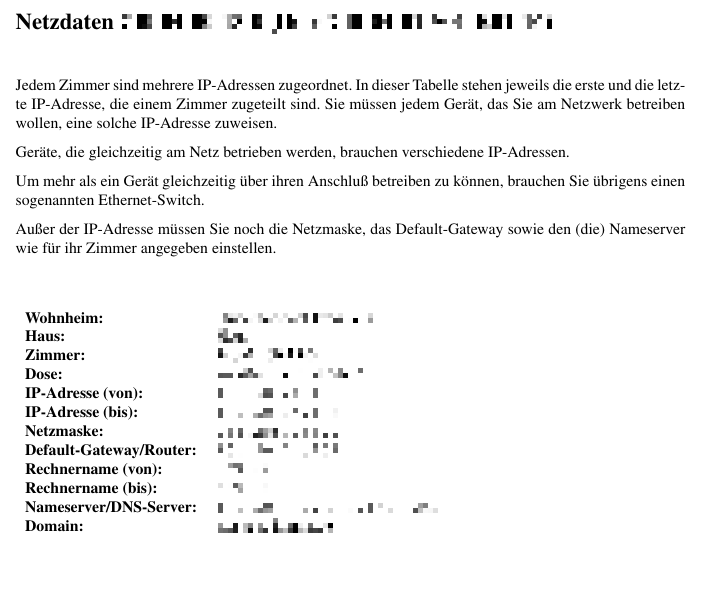
\includegraphics[width=\linewidth]{Bilder/ip_zettel}
%  \caption{Bildunterschrift}
\end{minipage}

\subsection{Verbinden eines Computers oder eines Routers mit der Netzwerkdose}
Ein Computer kann entweder direkt über ein LAN-Kabel mit der Netzwerkdose verbunden oder es kann ein Router dazwischen geschaltet werden.
Im Regelfall funktioniert dabei nur die \textbf{linke} Dose, die auch oft entsprechend markiert ist. 
Um auch WLAN verwenden zu können und für die Verwendung von mehreren Geräten ist langfristig die Nutzung eines Routers zu empfehlen.

LAN-Kabel und Router können im Handel oder als Mitglied auch beim \StuStaNet{} während der Sprechstunde (siehe weiter unten) erworben werden.

Das Einrichten der Internetanbindung besteht somit aus folgenden Teilen:
\begin{itemize}
	\item Anschluss des Routers oder Computers an die Netzwerkbuchse (im Regelfall der linke entsprechend auch markierte Stecker)
	\item Konfiguration der Netzwerkeinstellungen bzw.\@ IP-Adressen des Routers oder Computers, wenn direkt per LAN-Kabel angeschlossen in Kapitel~\ref{section_netzweradresse}
	\item (Nur für Nicht-Mitglieder,) Eintragen des Proxyservers bzw. -skripts im Browser auf allen Geräten bzw. Programmen in Kapitel~\ref{proxy}
\end{itemize}
Falls der Router mit den Netzwerkeinstellungen konfiguriert wurde, dürfen die IP-Adressen nicht auch auf dem Computer oder Smartphone eingestellt werden!
Zur Kontrolle, ob die Einrichtung erfolgreich war, kann man die folgenden Seiten aufrufen \mbox{\url{http://selftest.stustanet.de}}, \mbox{\url{https://wiki.stusta.de}} und \mbox{\url{http://neverssl.com}} aus dem Zimmernetzwerk (nicht dem Handynetz!) ausprobieren.
Weitere Hilfen gibt es auf \mbox{\url{https://stustanet.de/de/support/}}.

\subsection{Für Nicht-Mitglieder}
Falls man nicht Mitglied beim StuStaNet ist, muss man für jedes Gerät das im Zimmer benutzt werden soll entweder das Proxyskript verwenden (empfohlen) oder manuell den Proxyserver einstellen.
Nicht alle Programme unterstützen dabei die globalen Proxy-Einstellungen des Betriebssystems und unter Umständen müssen diese auch für einzelne Programme separat eingestellt werden.
\\
\\
\noindent\begin{minipage}{\textwidth}

\subsection{Übersicht Netzwerkeinstellungen mit den jeweiligen Proxy-Konfigurationen}
\label{subsec_settings}
Pro Anschluss stehen 8 IP-Adressen zur Verfügung. Der jeweilige Adressbereich ist auf der Netzwerkdose vermerkt oder auf dem Zettel mit den IP-Adressen aus Punkt~\ref{ip_sheet} zu finden.

\begin{center}
  \begin{tabularx}{\linewidth}{lXp{.2\linewidth}}
    \textbf{Einstellung} & \textbf{Wert} & \textbf{Beispiel} \\
    \midrule
    IP-Adresse & \nolinkurl{10.150.xxx.yyy} - \nolinkurl{10.150.xxx.zzz}, \newline 8 Adressen stehen zur Auswahl & \nolinkurl{10.150.243.16} – \nolinkurl{10.150.243.23} \\
    \hline
    Netzmaske/Subnetzmaske & \nolinkurl{255.255.255.0} & \\
    \hline
    Subnetzpräfixlänge & \nolinkurl{24} & \\
    \hline
    Standardgateway & \nolinkurl{10.150.xxx.254} \newline (Die ersten drei Blöcke wie IP-Adresse, der vierte Block \nolinkurl{254}) & \nolinkurl{10.150.243.254} \\
    \hline
    DNS-Server (Nameserver) & \nolinkurl{10.150.127.2} \newline \nolinkurl{10.150.125.2} & \\
    \hline
    DNS-Suffix (Domainname) & \nolinkurl{stusta.mhn.de} & \\
    \hline
    Proxyskript &{\nolinkurl{http://wpad.stusta.mhn.de/proxy.pac}} & \\ 
    \hline
    Proxyserver (manuell) & {\nolinkurl{http://proxy.stusta.mhn.de:3128}} & \\ 
    \bottomrule
  \end{tabularx}
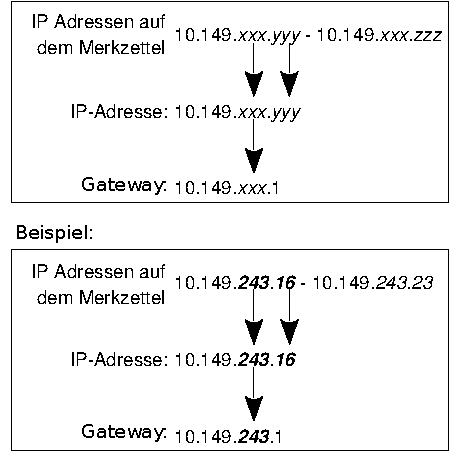
\includegraphics[width=0.4\linewidth,keepaspectratio]{Bilder/IP_Gerneric}
\end{center}
\end{minipage}

\newpage

\section{Konfiguration IP-Einstellungen}
\label{section_netzweradresse}
Hier sind die IP-Daten aus dem vorherigen Kapitel~\ref{sec:general} notwendig.
\subsection{Router}
Die Konfiguration der IP-Adressen auf dem Router ist modellabhängig.
Auf der folgenden Seite haben wir Schlagworte gesammelt, um in der Routeranleitung die richtigen Abschnitte zu finden.

\url{https://stustanet.de/de/support/router_instructions/}

Eine Anleitung zur Verbindung des Computers mit dem Router ist in der Anleitung des Routerherstellers zu finden.

Bei Benutzung eines Routers ist es nicht notwendig, die IP-Adressen auch auf den Endgeräten einzurichten wie es im Rest von Kapitel~\ref{section_netzweradresse} beschrieben ist, sondern nur auf dem Router.
Bei Nicht-Mitglieder ist die Proxykonfiguration auf den Endgeräten trotzdem noch notwendig, aber nicht auf dem Router.

\subsection{Konfiguration mit LAN-Kabel Computer (nur ohne Router notwendig)}
\subsubsection*{IP-Einstellungen LAN für Windows 10}
\begin{minipage}{0.57\textwidth}
\begin{enumerate}
	\item Klicken Sie auf das Windowssymbol in der unteren linken Ecke und anschließend auf \emph{Einstellungen}
	\item Klicken Sie auf \textit{Netzwerk- und Internet}.
	Scrollen Sie nach unten bis \textit{Netzwerk- und Freigabecenter} und klicken Sie auf diesen Punkt. Wählen Sie in der linken Spalte den Punkt \textit{Adaptereinstellungen ändern} aus.
	Sollten Sie diesen Punkt nicht finden, können Sie auch in der Suchzeile rechts oben nach \glqq Adaptereinstellungen ändern\grqq suchen.
    \item Ihnen sollten nun mehrere Netzwerkverbindungen aufgelistet sein. Klicken Sie mit der \textbf{rechten} Maustaste auf \textit{Ethernet} und klicken Sie auf \textit{Eigenschaften}.
    \item Markieren Sie den Eintrag \textit{Internetprotokoll Version 4 (TCP/IPv4)} und klicken Sie danach auf Eigenschaften.
    \item Jetzt geben Sie
    \begin{itemize}
    	\item IP-Adresse
    	\item Subnetzmaske
    	\item (Standart-)Gateway
    	\item Bevorzugter DNS
    	\item Alternativer DNS
    \end{itemize}
	ein.
    \item Klicken Sie auf \textit{Erweitert} und wählen im folgenden Dialog den Reiter DNS aus. Tragen Sie im Feld DNS-Suffix für diese Verbindung \textbf{stusta.mhn.de} ein.
    \item Bestätigen mit \textit{OK}.
\end{enumerate}
\end{minipage}
\hfill
\begin{minipage}{0.4\textwidth}
	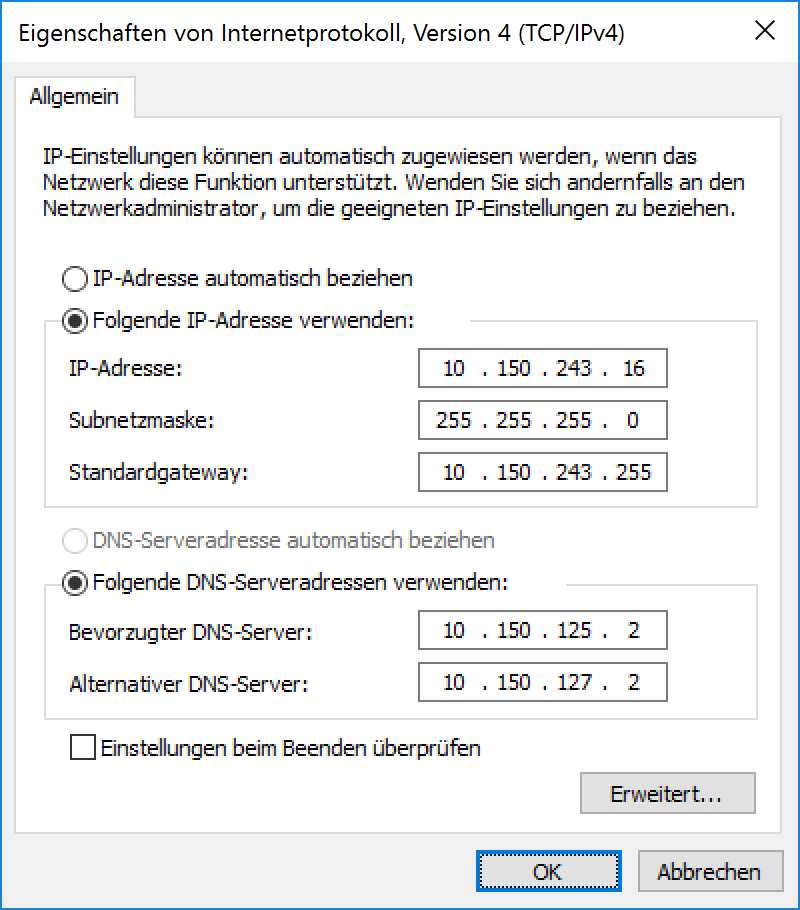
\includegraphics[width=\textwidth]{Bilder/IP_Windows}
	%  \caption{Bildunterschrift}
\end{minipage}%

\subsubsection*{IP-Einstellungen LAN für Windows 11}
\begin{minipage}{0.57\textwidth}
\begin{enumerate}
	\item Gehen Sie in den rechts gelb markierten Feldern zu \textit{Einstellungen} $\rightarrow$ \textit{Netzwerk und Internet} $\rightarrow$ \textit{Ethernet} $\rightarrow$ Bei \textit{IP-Zuweisung} klicke \textit{Bearbeiten}.
	\item Ändere das Dropdown-Menü zu \textit{Manuell}.
	\item Setzen Sie die Checkbox \textit{IPv4} auf \textit{Ein}.
	\item Jetzt tragen Sie in die rechts blau markierten Felder
		\begin{itemize}
			\item IP-Adresse
			\item Subnetzmaske
			\item Gateway
			\item Bevorzugter DNS
			\item Alternativer DNS
		\end{itemize}
	ihres Zimmers von Punkt~\ref{ip_sheet} ein.
	\item Bestätige mit \textit{Speichern}.
\end{enumerate}
\end{minipage}
\hfill
\begin{minipage}{0.4\textwidth}
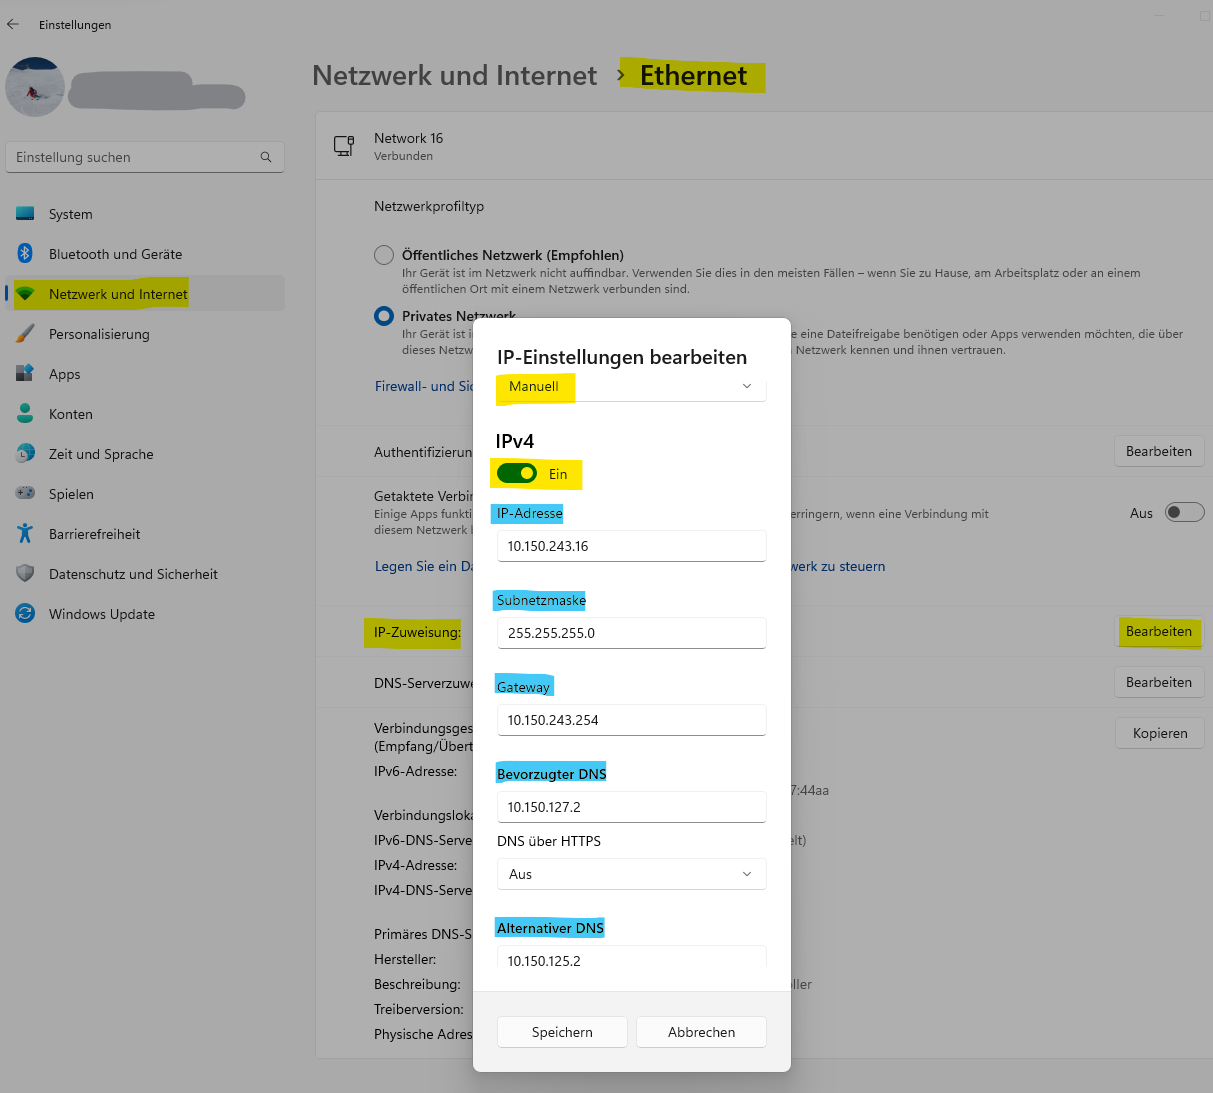
\includegraphics[width=\linewidth]{Bilder/Win11/ip_win11_de}
\end{minipage}

\subsubsection*{IP-Einstellungen LAN für Linux}

Beispiel für \textit{Networkmanager}.
Kann abweichen je nach Distribution, sollte aber im Kern ähnlich sein.

\begin{minipage}{0.57\textwidth}
\begin{enumerate}
	\item Öffnen Sie die Netzwerkkonfiguration durch Klick auf \emph{System} $\rightarrow$ \emph{Einstellungen} $\rightarrow$ \emph{Netzwerkkonfiguration}.
	\item Markieren Sie nun im Reiter Kabelgebunden den entsprechenden Eintrag Ihrer Netzwerkkarte (im Normalfall \emph{eth0}) und klicken Sie auf den Button \emph{Bearbeiten}.
	\item Gehen Sie zum Reiter \emph{IPv4-Einstellungen} und setzen Sie Methode auf \emph{Manuell}.
	\item Unter \emph{Adressen} klicken Sie auf den Button \emph{Hinzufügen}.
	\item Jetzt geben Sie
	\begin{itemize}
		\item IP-Adresse
		\item Subnetzmaske
		\item Gateway
		\item DNS
		\item Suchdomäne
	\end{itemize}
	ein.
	\item Bestätigen Sie mit \emph{OK} und schließen Sie das Fenster für die Netzwerkeinstellungen.
\end{enumerate}
\end{minipage}
\hfill
\begin{minipage}{0.4\textwidth}
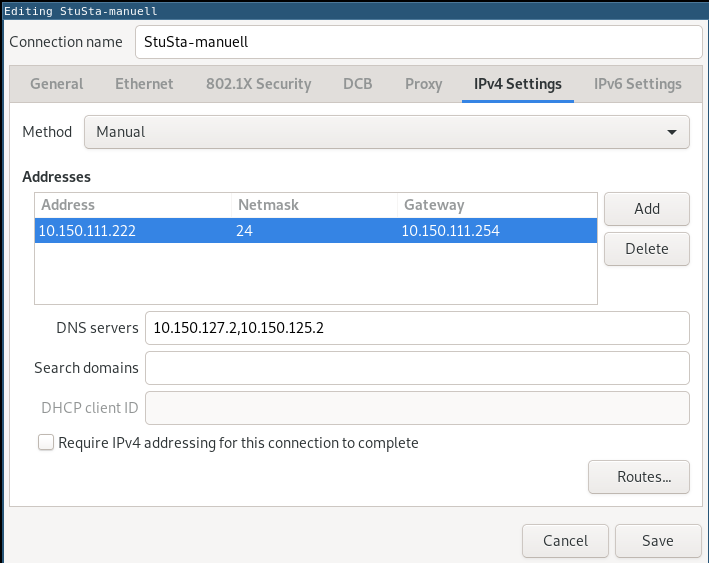
\includegraphics[width=\linewidth]{Bilder/IP_Ubuntu_neu}
\end{minipage}

\subsubsection*{IP-Einstellungen LAN für MacOS}

\begin{minipage}{0.57\textwidth}
\begin{enumerate}
    \item Öffnen Sie die Netzwerkkonfiguration durch Klick auf \emph{Apfel} (oben links) und wählen dann \emph{Systemeinstellungen} $\rightarrow$ \emph{Netzwerk} aus.
    \item Markieren Sie nun das Netzwerkgerät \emph{Ethernet}.
    \item Setzen Sie das Feld \emph{IPv4 Konfigurieren} auf \emph{Manuell}.
    \item Jetzt geben Sie
    \begin{itemize}
    	\item IP-Adresse
    	\item Netzmaske/Teilnetzmaske
    	\item Gateway/Router
    	\item DNS
    	\item Suchdomäne
    \end{itemize}
	in den entsprechenden Feldern ein.
	\item Bestätigen Sie mit \emph{Anwenden}.
\end{enumerate}
\end{minipage}
\hfill
\begin{minipage}{0.4\textwidth}
	\centering
	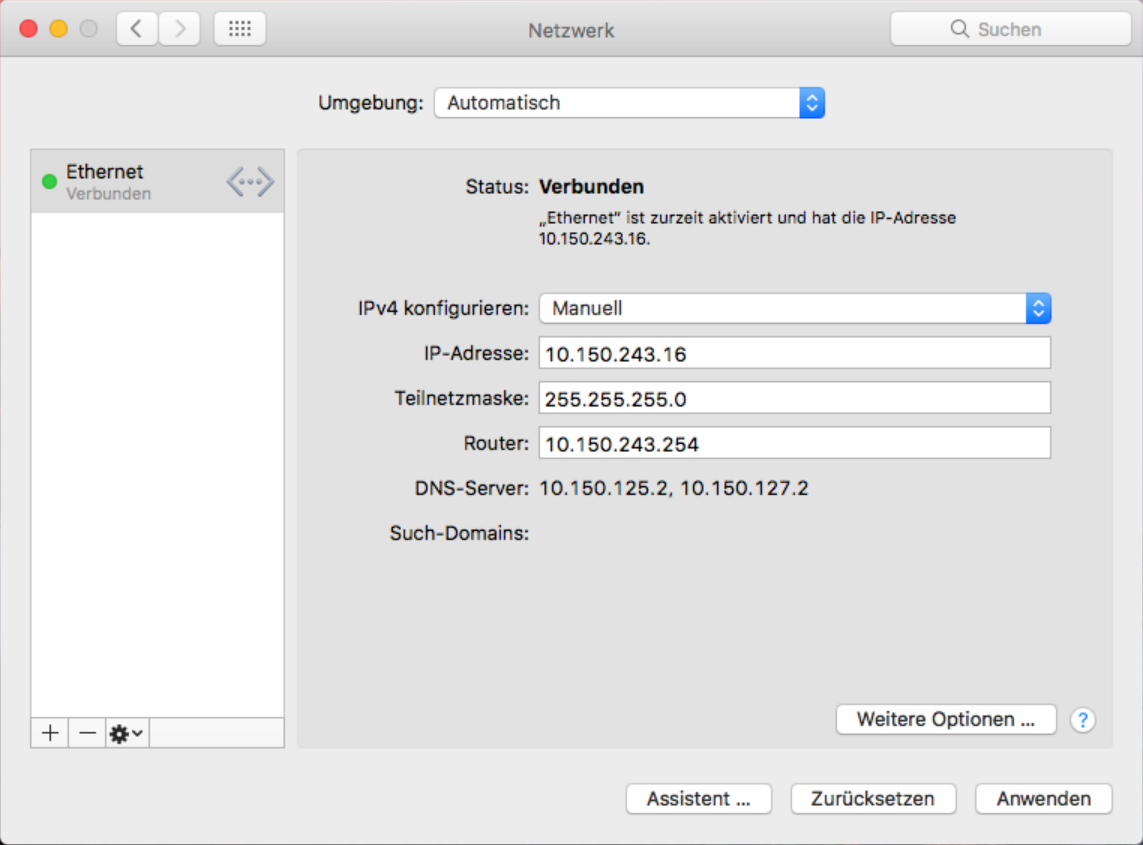
\includegraphics[width=\linewidth,keepaspectratio]{Bilder/IP_MAC}
\end{minipage}

\subsubsection*{IP-Einstellungen LAN für MacOS (ab Ventura)}

\begin{minipage}{0.57\textwidth}
	\begin{enumerate}
		\item Öffnen Sie die Netzwerkkonfiguration durch Klick auf \emph{Apfel} (oben links) und wählen dann \emph{Systemeinstellungen} $\rightarrow$ \emph{Netzwerk} aus.
		\item Wählen Sie nun ihren LAN-Adapter bzw. Dock aus.
		\item Klicken Sie auf \textit{Details}.
		\item Gehen Sie auf den Reiter \textit{TCP/IP}.
		\item Wählen Sie beim Feld \textit{IPv4 Konfigurieren} die Option \textit{Manuell}.
		\item Jetzt geben Sie
		\begin{itemize}
			\item IP-Adresse
			\item Netzmaske/Teilnetzmaske
			\item Gateway/Router
		\end{itemize}
	ein.
	\item Als Nächstes wählen Sie den Reiter \textit{DNS} aus.
	\item Fügen Sie beim \textit{DNS-Server} jeweils einzeln mittels \textbf{+} die beiden \textit{DNS-Server} hinzu.
	\item Fügen Sie bei \textit{Suchdomäne} mittels \textbf{+} die \textit{Suchdomäne} hinzu.
	\item Bestätigen Sie mit \emph{Anwenden}.
	\end{enumerate}
\end{minipage}
\hfill
\begin{minipage}{0.4\textwidth}
	\centering
	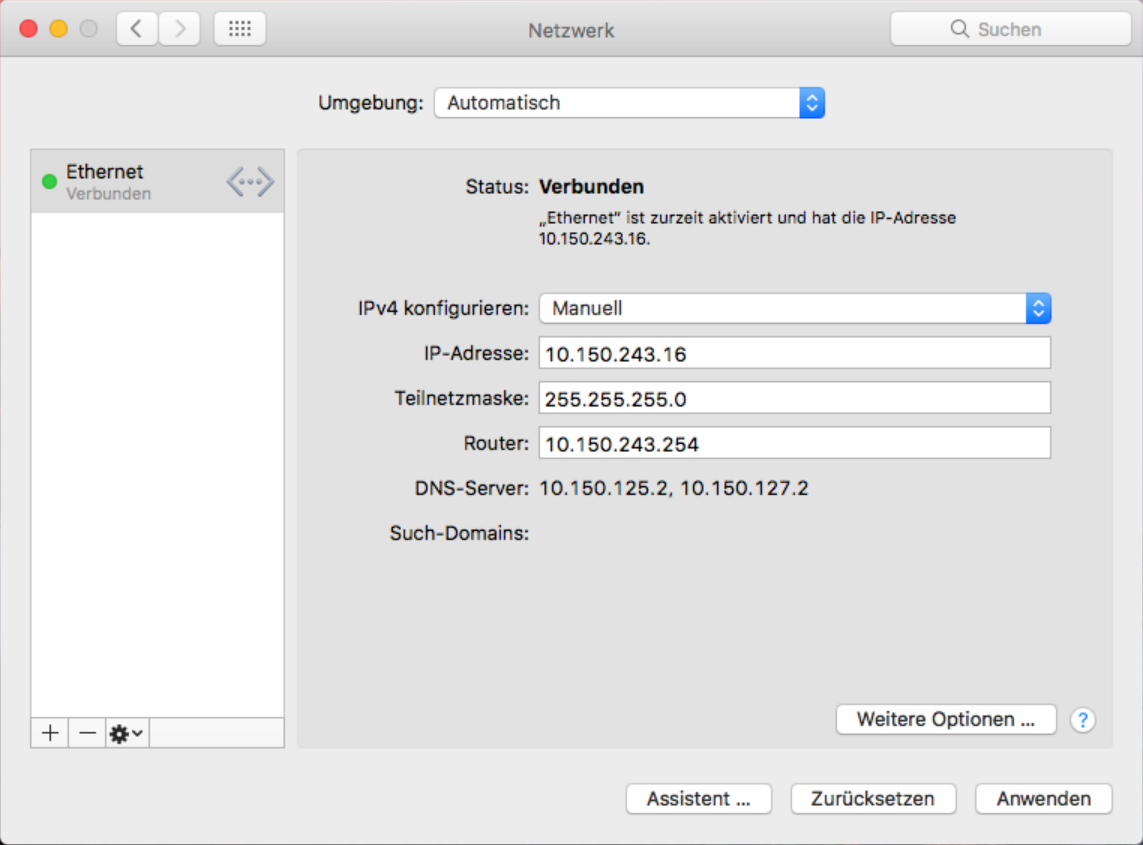
\includegraphics[width=\linewidth,keepaspectratio]{Bilder/IP_MAC}
\end{minipage}

\section{Proxyeinstellungen (nur für Nicht-Mitglieder notwendig)}
\label{proxy}

\subsection*{Globaler Proxy für Windows 10/11}
\begin{enumerate}
	\item Wähle \textit{Einstellungen} $\rightarrow$ \textit{Netzwerk und Internet} $\rightarrow$ \textit{Proxy}.
	%	\item Deaktivieren Sie die Option \emph{Einstellungen automatisch erkennen}.
	\subitem \textbf{Nur Windows 11:} Klicke bei \textit{Setupskript verwenden} auf den Button  \textit{Einrichten}.
	
	\setcounter{enumi}{1}
	\item Setzen Sie \textit{Setupskript verwenden} auf \textit{Ein}.
	\item Tragen Sie als Skriptadresse die \textit{.pac Proxyskript-Adresse} ihres Zimmers ein.
	\item Bestätige Sie mit \textit{Speichern}.
\end{enumerate}

\begin{figure}[h]
	\centering
	\begin{minipage}{.55\textwidth}
		\centering
		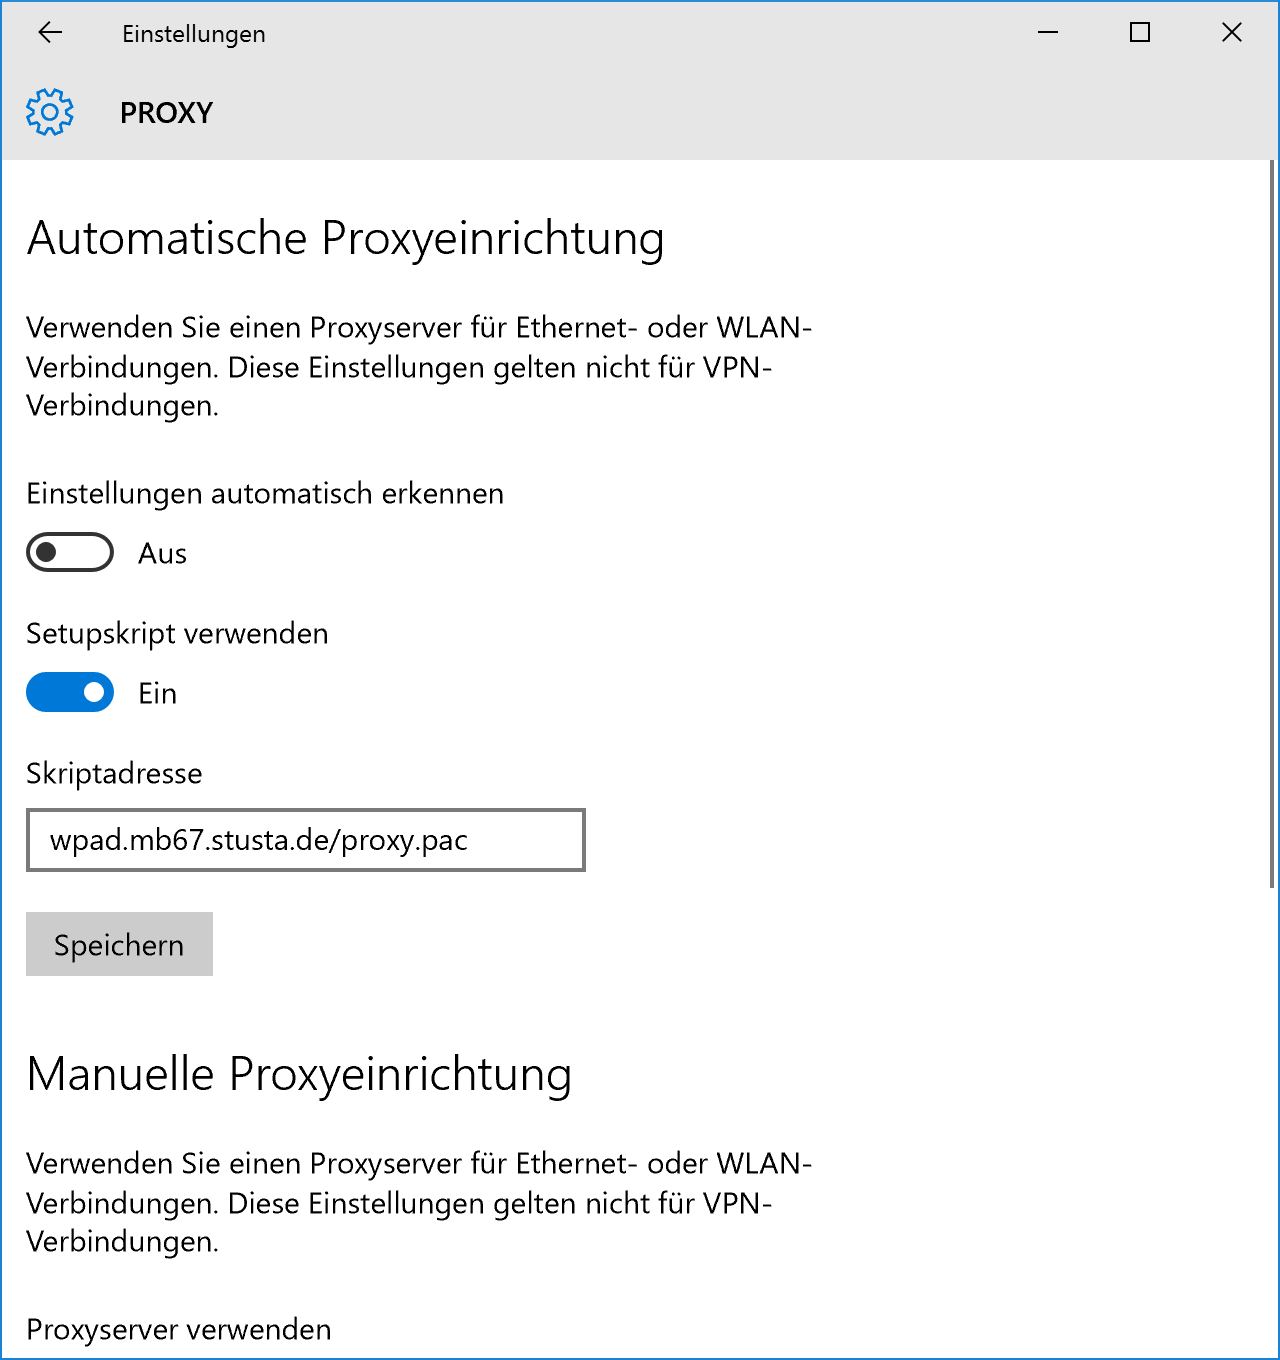
\includegraphics[height=.20\textheight]{Bilder/Proxy_Edge}
	\end{minipage}
	\begin{minipage}{.30\textwidth}
		\centering
		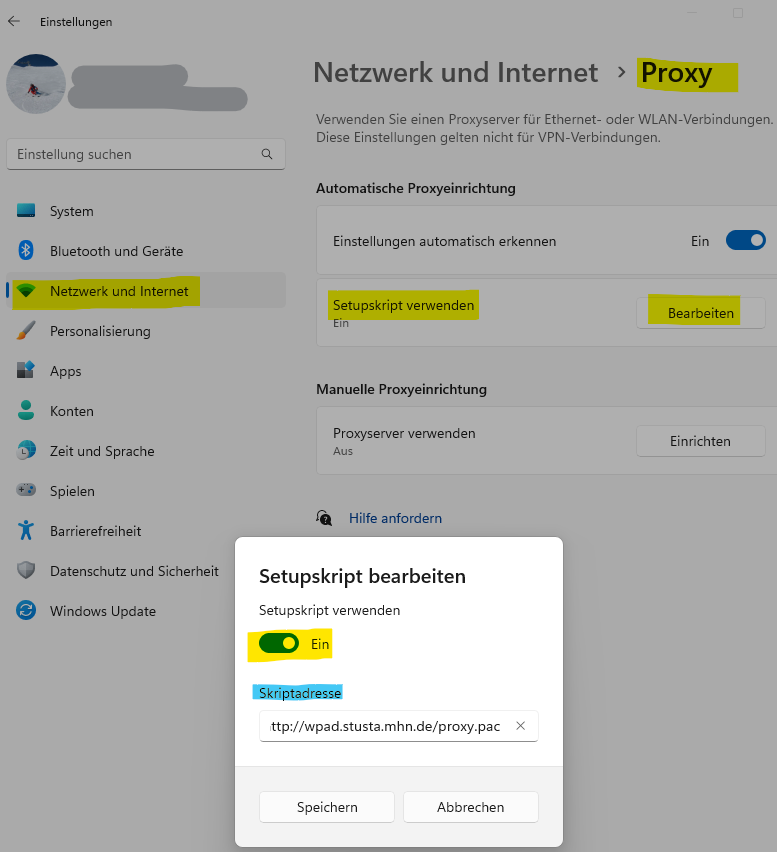
\includegraphics[height=.20\textheight]{Bilder/Win11/proxy_win11_de}
	\end{minipage}
\end{figure}

\subsection*{Globaler Proxy für Linux}
Kann abweichen je nach Distribution, sollte aber im Kern ähnlich sein.
\begin{enumerate}
	\item Öffnen Sie die Netzwerk-Proxy-Einstellungen durch Klick auf \emph{System} $\rightarrow$ \emph{Einstellungen} $\rightarrow$ \emph{Netzwerk-Proxy}.
	\item Hier markieren Sie ganz unten die Option \emph{Automatische Proxy-Konfiguration} und tragen bei URL für Auto-Konfiguration: die \textit{.pac Proxyskript-Adresse} ihres Zimmers ein. Schließen Sie das Fenster. 
\end{enumerate}

\subsection*{Globaler Proxy für MacOS}
\begin{enumerate}
	\item Öffnen Sie mit dem Button \emph{Weitere Optionen...} im voherigen Dialog die Detaileinstellungen und wechseln sie auf die Registerkarte \emph{Proxies}.
	\item Setzen sie bei Zu konfigurierendes Protokoll vor Autom. Proxy-Konfiguration einen Hacken und tragen rechts bei URL die \textit{.pac Proxyskript-Adresse} ihres Zimmers ein. Schließen Sie die Detaileinstellungen mit OK und bestätigen Sie erneut mit Anwenden. Sie können die Netzwerkeinstellungen jetzt schließen.
\end{enumerate}

\subsection*{Globaler Proxy Android}
Bei den verschiedenen Herstellern kann das Interface leider abweichen.
Wenn du Probleme hast, kann du versuchen im Internet nach Anleitungen für dein Handymodell in Verbindung mit den Schlagworten \textit{Proxy Einrichtung} suchen.

\subsubsection*{Google Pixel Android 12}
\begin{enumerate}
	\item Öffnen Sie die WLAN-Einstellungen.
	\item Klicken Sie auf das Zahnrad neben dem Namen deines WLAN-Netzwerkes.
	\item Klicken Sie auf das Stiftsymbol am oberen rechten Bildschirmrand.
	\item Aktivieren Sie das Drop-Down-Menü \textit{Erweiterte Optionen}.
	\item Wählen Sie unter \textit{Proxy} den Punkt \textit{Automatische Proxykonfiguration}.
	\item Tragen Sie als \textit{PAC-URL} die \textit{.pac Proxyskript-Adresse} ihres Zimmers ein.
	\item Bestätige Sie mit \textit{Speichern}.
\end{enumerate}

\begin{figure}[h]
	\centering
	\begin{minipage}{0.20\textwidth}
		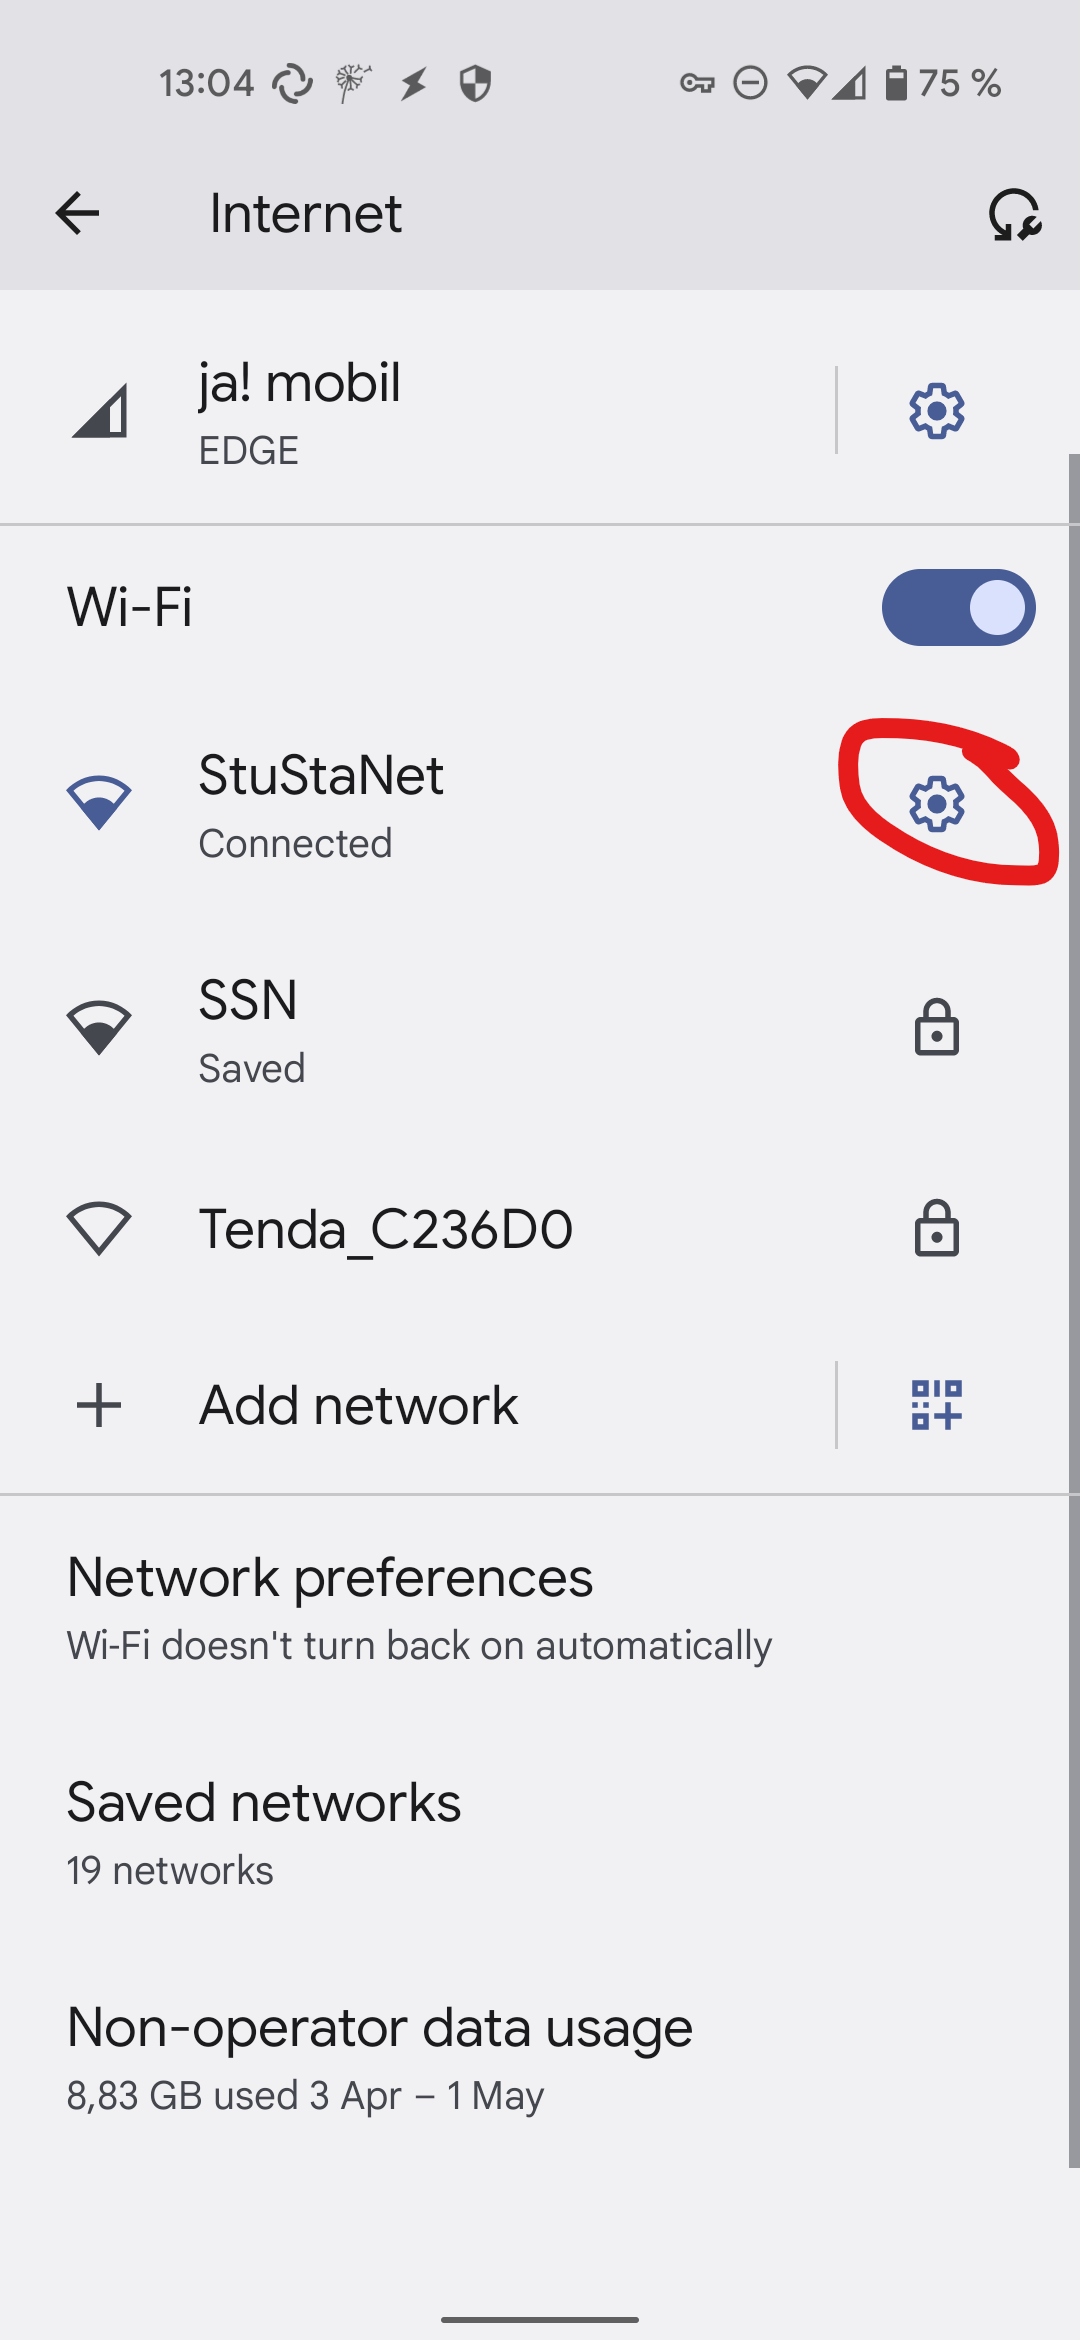
\includegraphics[width=0.7\linewidth,keepaspectratio]{Bilder/Android/android12_1}
	\end{minipage}
	\begin{minipage}{0.20\textwidth}
		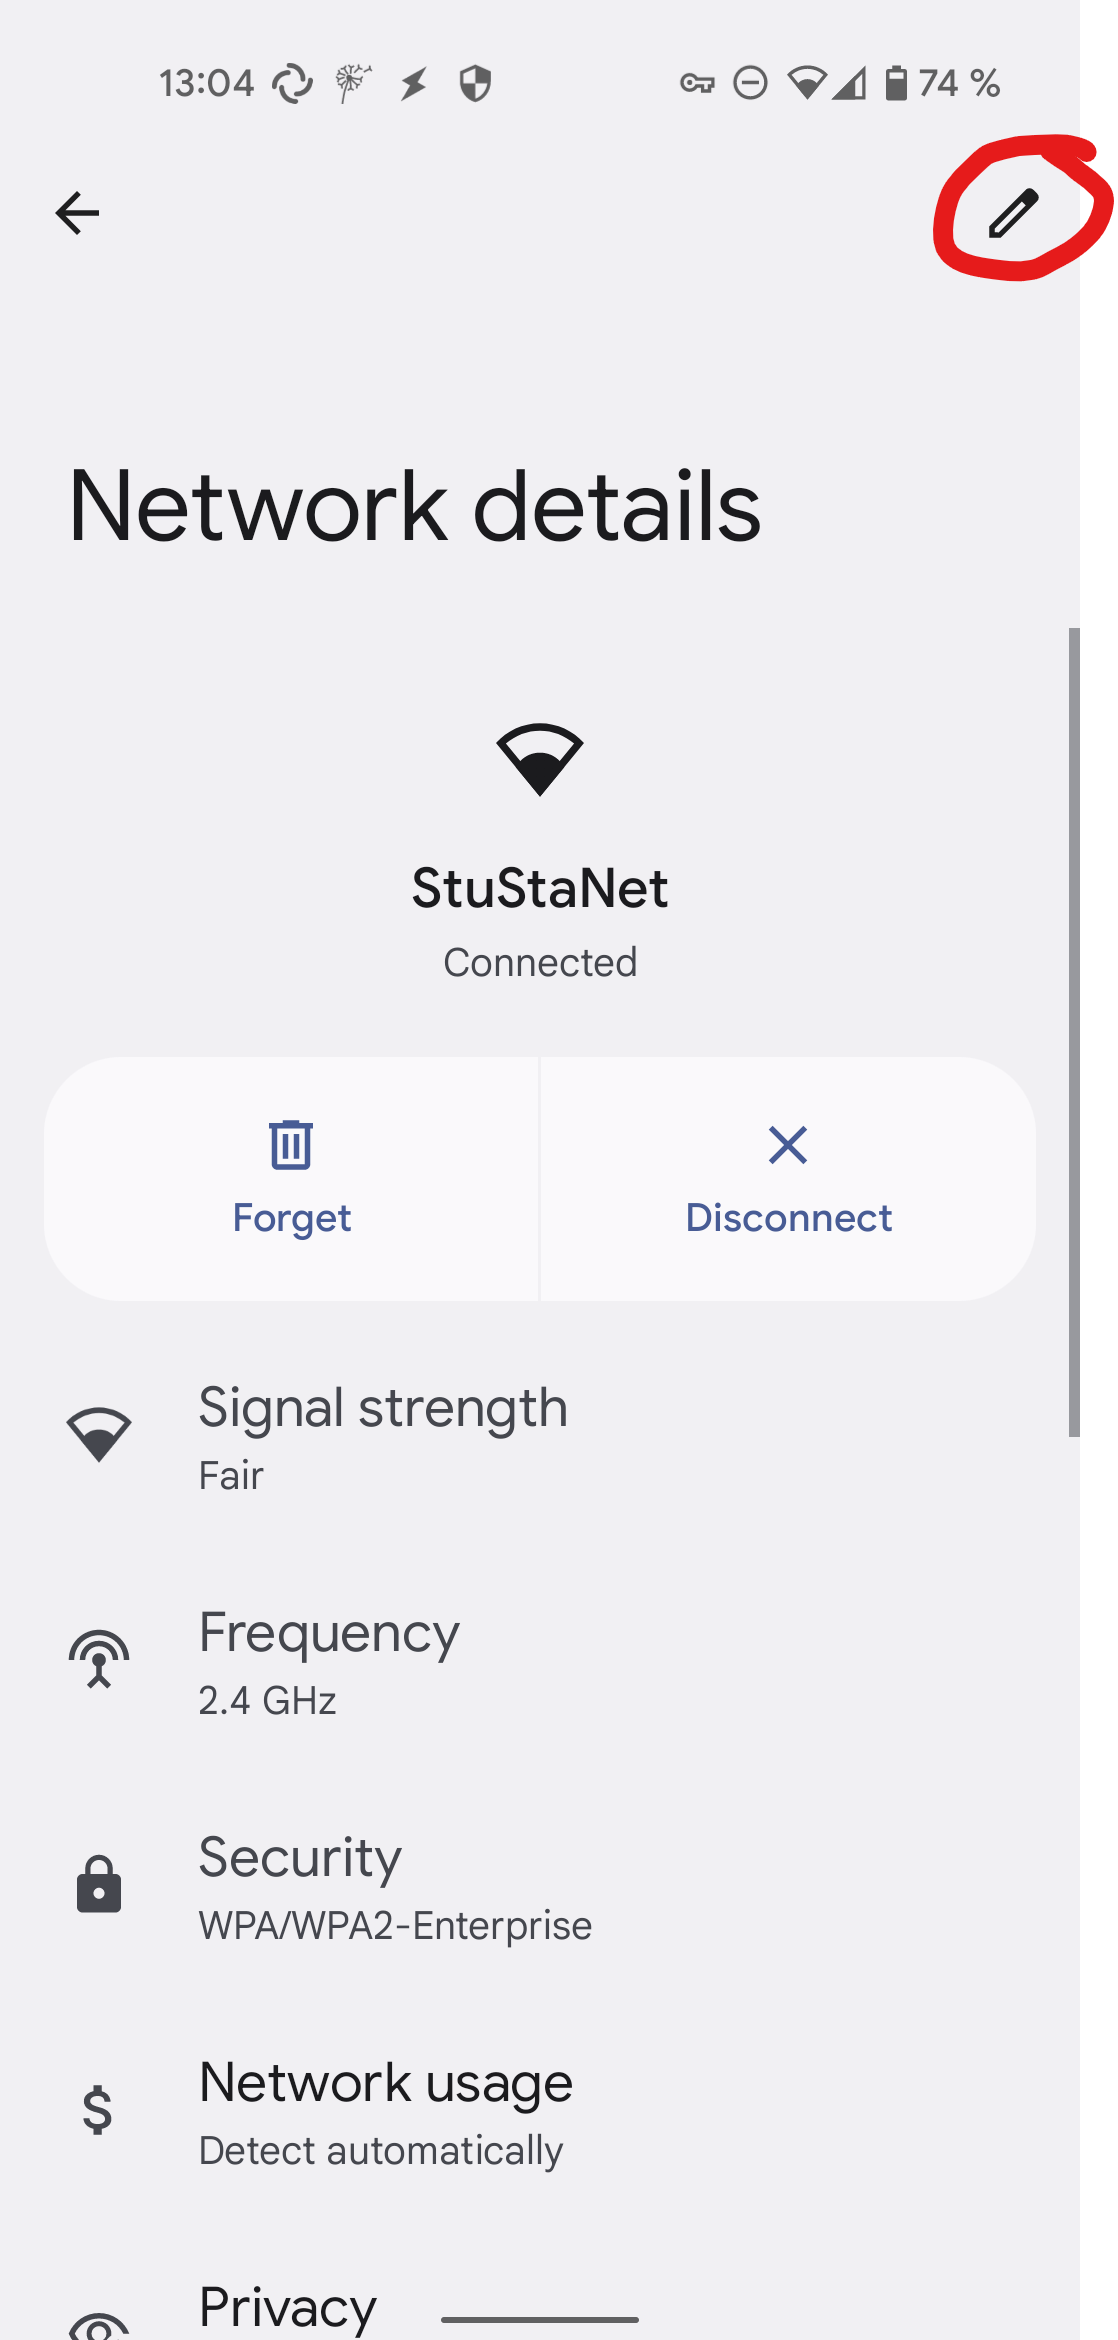
\includegraphics[width=0.7\linewidth,keepaspectratio]{Bilder/Android/android12_2}
	\end{minipage}
	\begin{minipage}{0.20\textwidth}
		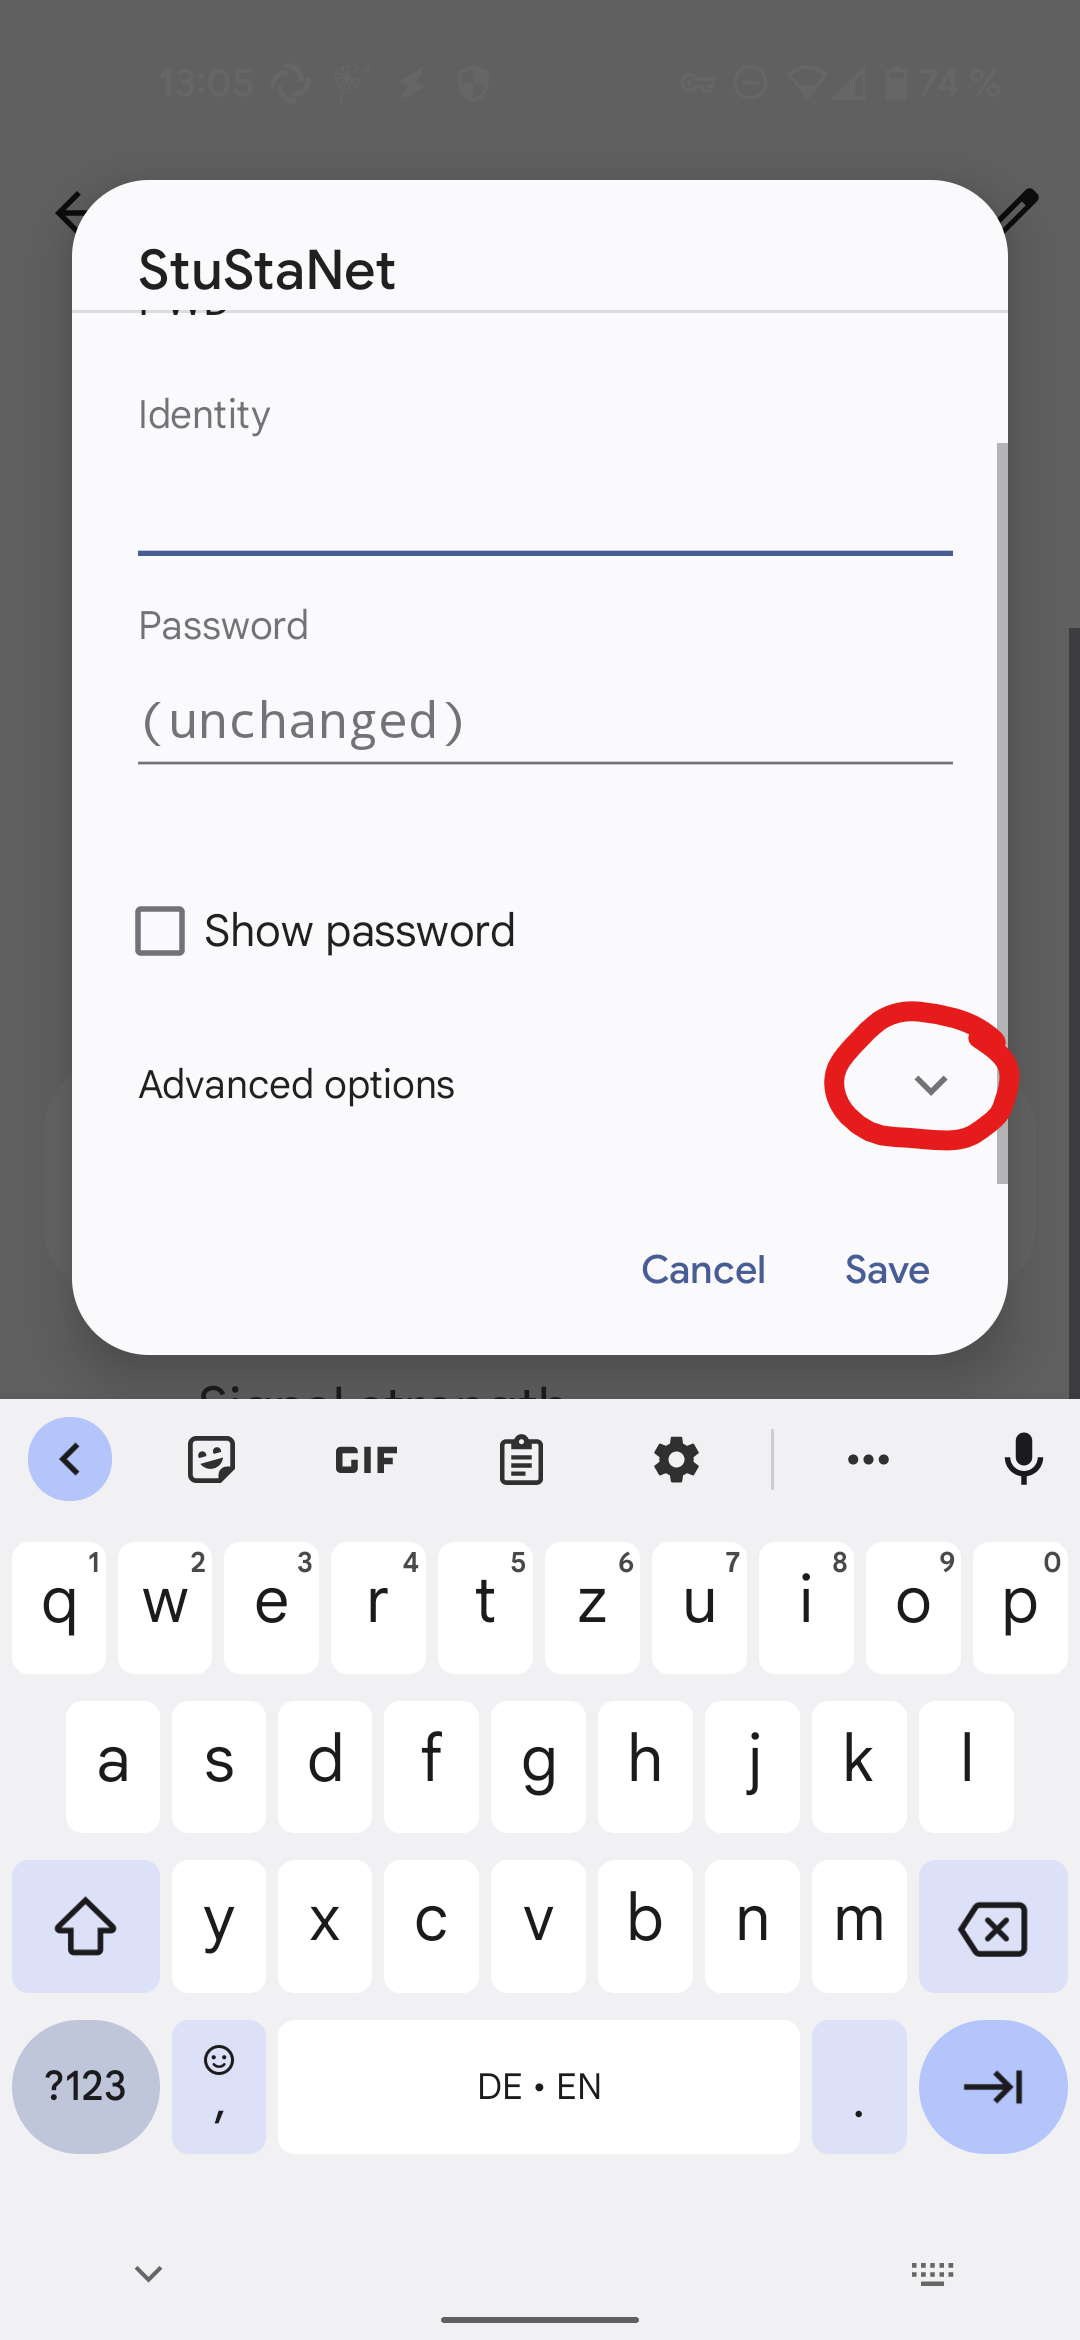
\includegraphics[width=0.7\linewidth,keepaspectratio]{Bilder/Android/android12_3}
	\end{minipage}
	\begin{minipage}{0.20\textwidth}
		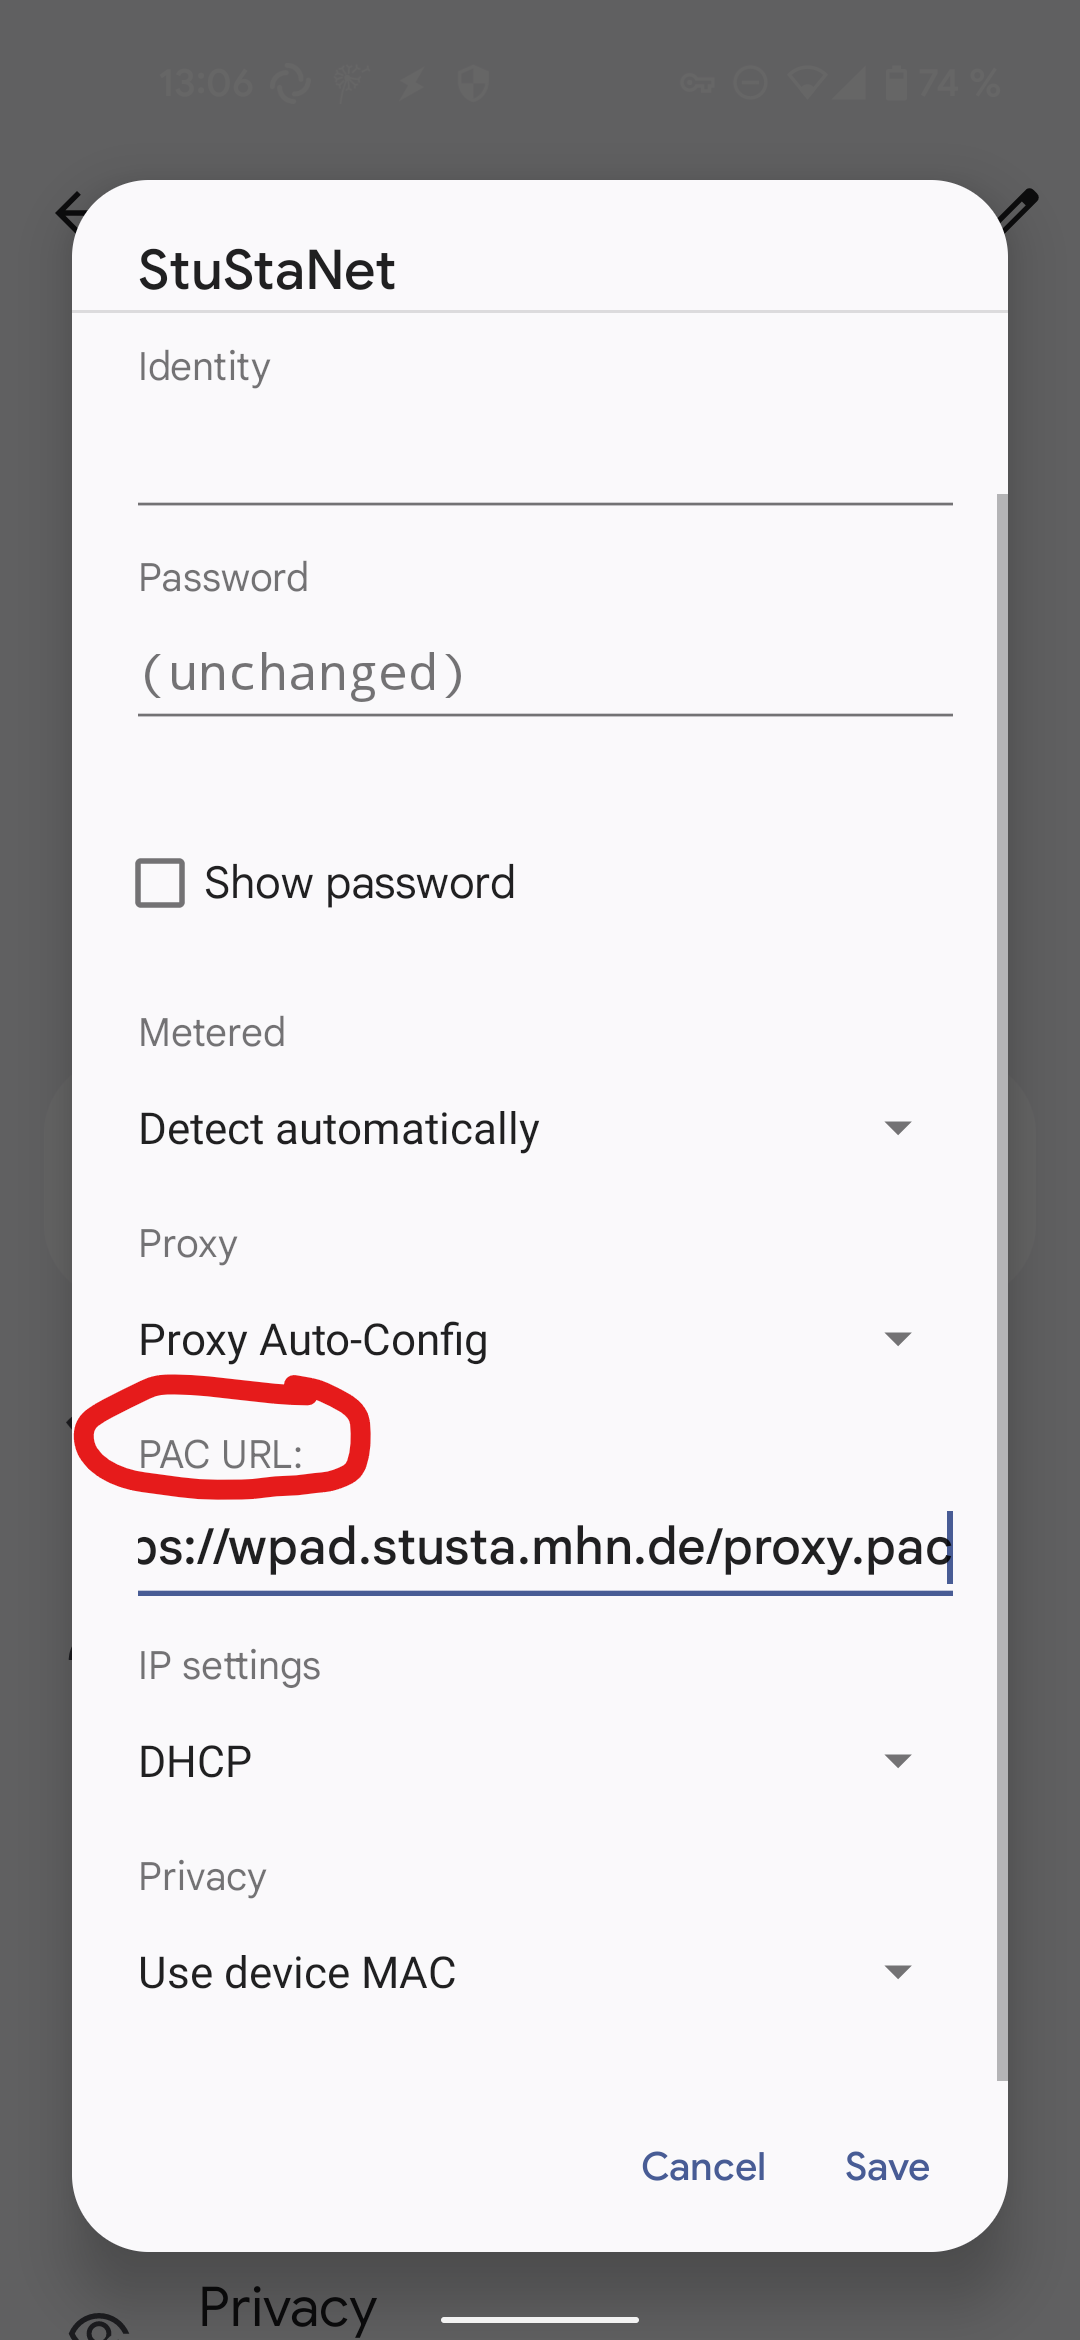
\includegraphics[width=0.7\linewidth,keepaspectratio]{Bilder/Android/android12_4}
	\end{minipage}
\end{figure}

\subsection*{Globaler Proxy andere Geräte}
Wenn du Probleme hast, kann du versuchen im Internet nach Anleitungen für dein Gerät in Verbindung mit den Schlagworten \textit{Proxy Einrichtung} suchen.

\subsection*{Proxy-Konfiguration im Browser}
\label{Proxy}

\subsubsection*{Mozilla Firefox}

\begin{minipage}{0.57\textwidth}
\begin{enumerate}
	\item Klicken Sie auf die 3 übereinanderliegenden Striche in der rechten oberen Ecke, wählen Sie danach \emph{Einstellungen}.
	\item Gehen Sie zum Punkt \emph{Verbindungs-Einstellungen} und wählen diesen aus.
	\item Markieren Sie den Punkt \emph{Automatische Proxy-Konfigurations-Adresse} und tragen Sie als automatische Proxy-Konfigurations-URL die \textit{.pac Proxyskript-Adresse} ihres Zimmers ein.
	\item Bestätigen Sie mit \textit{OK}.
\end{enumerate}
\end{minipage}
\hfill
\begin{minipage}{0.4\textwidth}
\centering
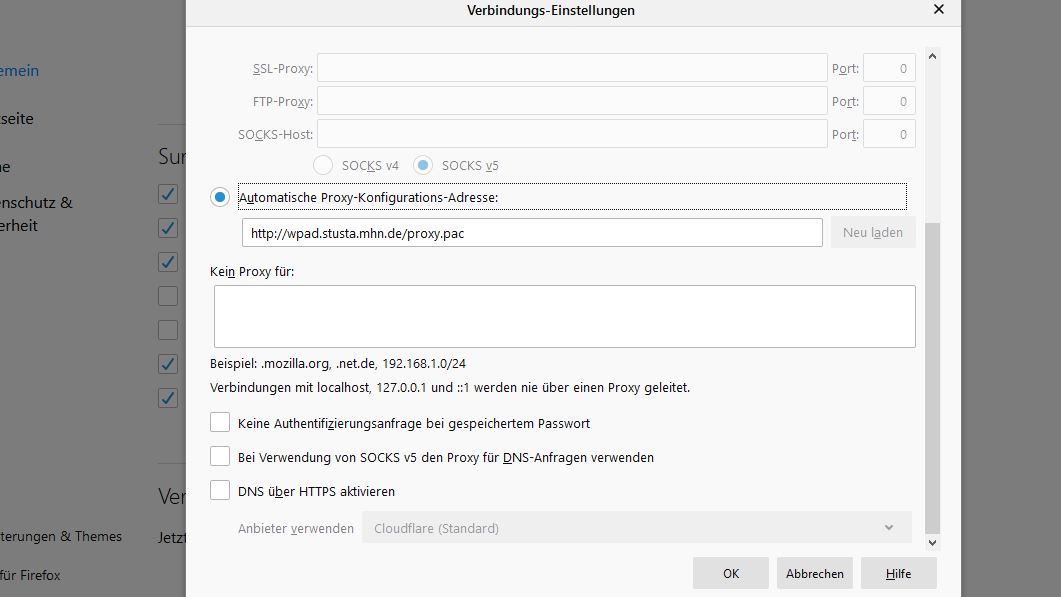
\includegraphics[width=\linewidth,keepaspectratio]{Bilder/Firefox_neu_proxy}
\end{minipage}

\subsubsection*{Google Chrome \& Microsoft Edge}
Diese Browser verwenden die Proxyeinstellungen des Betriebssystems.
Sieh dir dafür den passenden Abschnitt weiter oben an.

\section{Kontrolle \& Debugging}
Zur Kontrolle könnt ihr versuchen aus eurem Zimmeranschluss die folgenden Seiten aufzurufen.
\begin{itemize}
	\item \url{http://selftest.stustanet.de}
	\begin{itemize}
		\item Rudimentärer Selftest
	\end{itemize}
	\item \url{https://wiki.stusta.de}
	\begin{itemize}
		\item StuSta-Internes Wiki
		\item Bei Fehler Hinweis auf Problem bei IP-Konfiguration aus Kapitel~\ref{section_netzweradresse} oder dem Anschluss des Router/Computers aus Kapitel~\ref{sec:general}.
		\item Falls aufrufbar, aber andere Seiten nicht, Hinweis auf Probleme mit Proxykonfiguration aus Kapitel~\ref{proxy}.
	\end{itemize}
\end{itemize}

\end{document}
